\section{Working Mechanism of Wireless Sensing\label{sec:mechanism}}
\begin{figure} [t!]
       \centering
        \subfigure[]{
                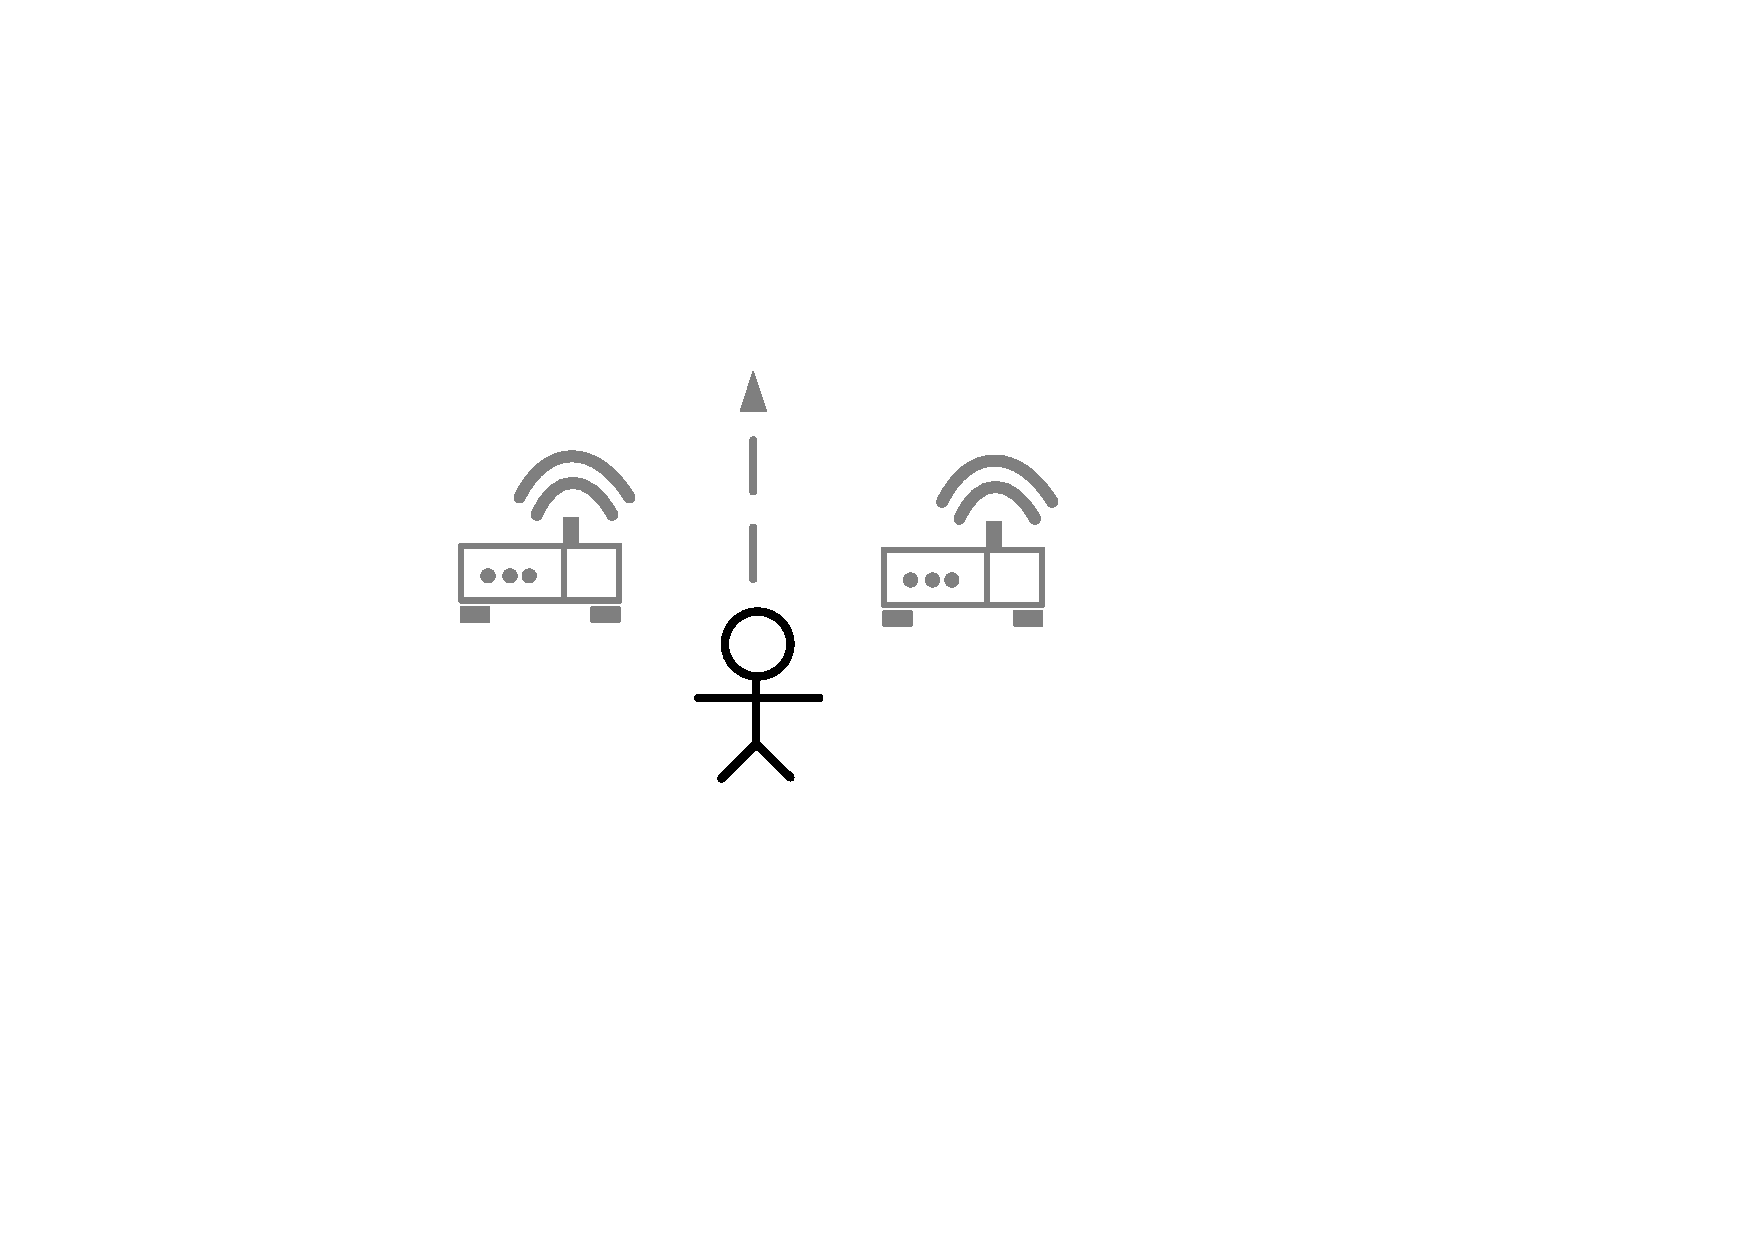
\includegraphics[width=0.22\textwidth]{figures/setup_example.pdf}
                \label{fig:scenario_1}
        }
        \subfigure[]{
                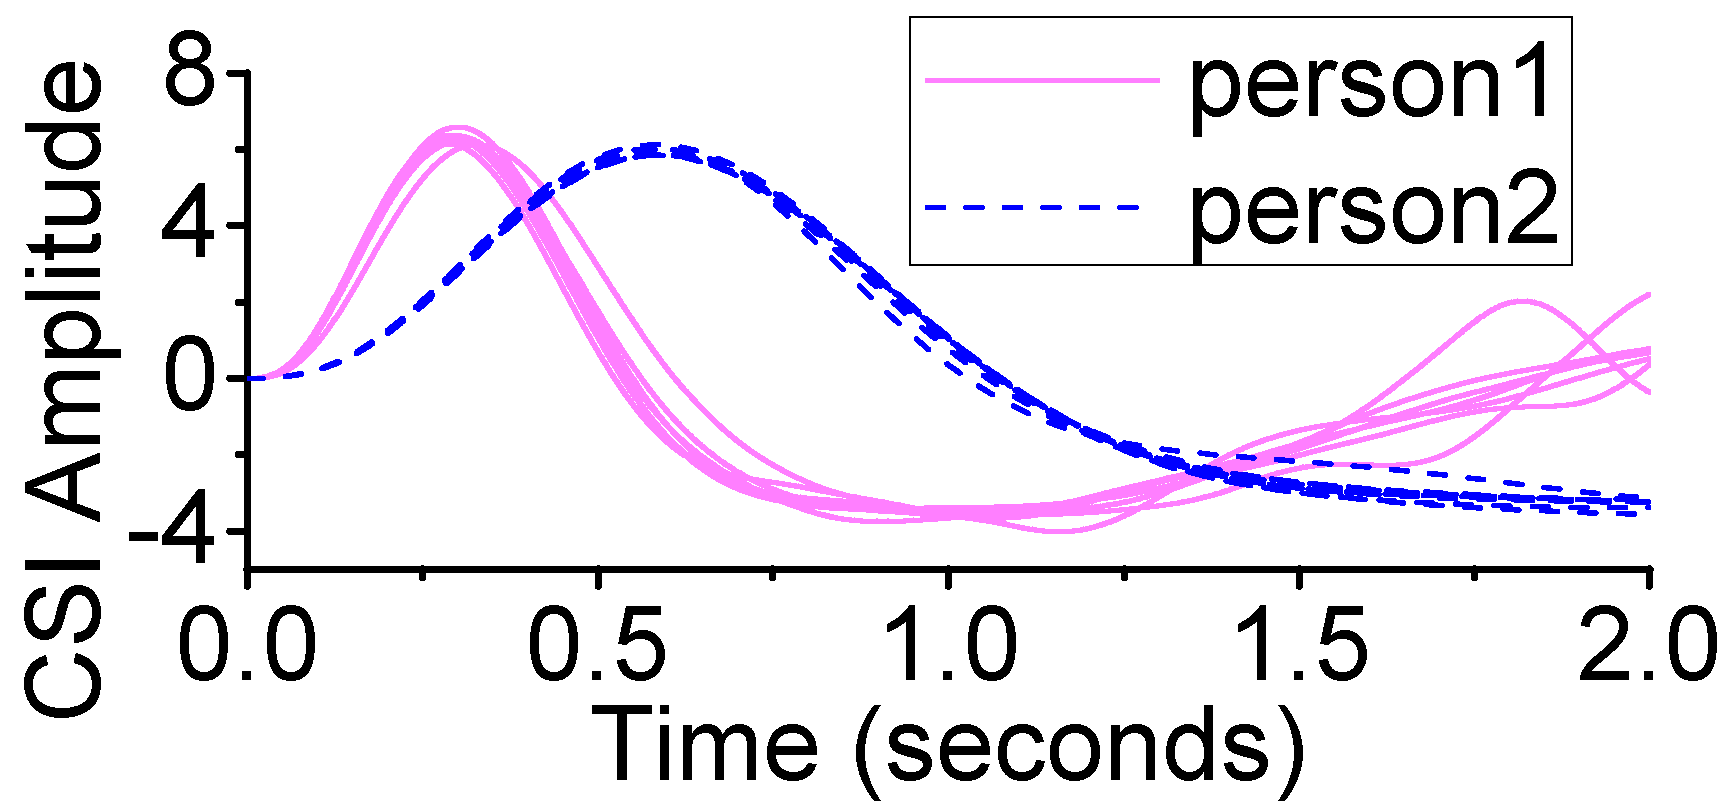
\includegraphics[width=0.22\textwidth]{figures//diff.pdf}
                \label{fig:csi_diff}
        }%
     \caption{The working mechanism of wirless sensing. (a) shows a typical set up where two wireless devices are deployed
     to collect the \CSI values when a user walks pass the devices. (b)  shows the measured \CSI  for two
     individuals, where the resulted \CSI amplitudes are relatively consistent for the same person across multiple walks, but are sufficiently different for different people.}
     \label{fig:csi_demo}
\end{figure}


\subsection{Working Example}
To illustrate how wireless sensing works, consider the gait identification scenario depicted in Figure~\ref{fig:scenario_1}. The sensing
task in this example is to identify which of a set of known users has walked pass the scene. Knowing this information allows one to -- for
example -- personalize the light setting of a smart home. Here, two wireless routers (a sender and a receiver) are used to measure how the
user's movement affect the wireless channel metric, such as the channel state information (\CSI) or received signal strength indicator
(\RSSI). The idea is that the wireless signal -- called ``multipath" -- will bounce off the wall, furniture, and human body, and the human
activity can lead to a subtle change on the attenuation and reflections of the signal; by measuring how the wireless signal is affected by
the activity and comparing the measurement against some pre-collected training data, one can infer what activity has been performed and by
whom.

Figure~\ref{fig:csi_diff} shows the measured \CSI amplitudes of two users in our scenario. In this case, each user walked through our scene
five times and the \CSI amplitude per walk is shown. This figure suggests that wireless channel metrics can be a useful means for user
identification, because the channel metric measurements for the same person is relatively consistent but is sufficiently different for the
two  people.

Note that although the setup and the sensing method would vary depending on the sensing task and the wireless signal to use, this example
shares many of the commonalities of wireless sensing, which demonstrates the underlying working principal of wireless sensing.
